\documentclass[12pt]{article}

% Pretty much all of the ams maths packages
\usepackage{amsmath,amsthm,amssymb,amsfonts}

% Allows you to manipulate the page a bit
\usepackage[a4paper]{geometry}

% Pulls the page out a bit - makes it look better (in my opinion)
\usepackage{a4wide}

% Removes paragraph indentation (not needed most of the time now)
\usepackage{parskip}

% Allows inclusion of graphics easily and configurably
\usepackage{graphicx}

% Provides ways to make nice looking tables
\usepackage{booktabs}

% Allows you to rotate tables and figures
\usepackage{rotating}

% Allows shading of table cells
\usepackage{colortbl}
% Define a simple command to use at the start of a table row to make it have a shaded background
\newcommand{\gray}{\rowcolor[gray]{.9}}

\usepackage{textcomp}

% Provides commands to make subfigures (figures with (a), (b) and (c))
\usepackage{subfigure}

% Typesets URLs sensibly - with tt font, clickable in PDFs, and not breaking across lines
\usepackage{url}

% Makes references hyperlinks in PDF output
\usepackage{hyperref}

% Provides ways to include syntax-highlighted source code
\usepackage{listings}
\lstset{frame=single, basicstyle=\ttfamily}

% Provides Harvard-style referencing
\usepackage{natbib}
\bibpunct{(}{)}{;}{a}{,}{,}

% Provides good access to colours
\usepackage{color}
\usepackage{xcolor}

% Simple command I defined to allow me to mark TODO items in red
\newcommand{\todo}[1] {\textbf{\textcolor{red}{#1}}}

% Allows fancy stuff in the page header
\usepackage{fancyhdr}
\pagestyle{fancy}

% Vastly improves the standard formatting of captions
\usepackage[margin=10pt,font=small,labelfont=bf, labelsep=endash]{caption}

% Standard title, author etc.
\title{Report: Sudoku}
\author{by	Karina Abramova,\\ Mikkel Bernt Buchvardt \\ and\\ Theodor Lars Nyholm Ommen}
\date{}
% Put text on the left-hand and right-hand side of the header
\fancyhead{}
\lhead{Sudoku}
\rhead{Abramova - Buchvardt - Ommen}
\chead{}

\usepackage{titletoc}

\renewcommand{\thepart}{\Alph{part}}

\renewcommand{\thesection}{\arabic{section}}
\renewcommand{\thesubsection}{\alph{subsection})}
\renewcommand{\thesubsubsection}{\alph{subsection}\alph{subsubsection})}

\titlecontents{chapter}
[2.65em]
{\addvspace{10pt}\bfseries}
{\contentslabel{2.3em}}
{\hspace*{-2.3em}}
{\space.\hfill\contentspage}


\definecolor{dkgreen}{rgb}{0,0.6,0}
\definecolor{gray}{rgb}{0.5,0.5,0.5}
\definecolor{mauve}{rgb}{0.58,0,0.82}

\lstset{frame=tb,
	language=Java,
	aboveskip=3mm,
	belowskip=3mm,
	showstringspaces=false,
	columns=flexible,
	basicstyle={\small\ttfamily},
%	numbers=left,
	numberstyle=\tiny\color{gray},
	keywordstyle=\color{blue},
	commentstyle=\color{dkgreen},
	stringstyle=\color{mauve},
	breaklines=true,
	breakatwhitespace=true,
	tabsize=3
}

\begin{document}


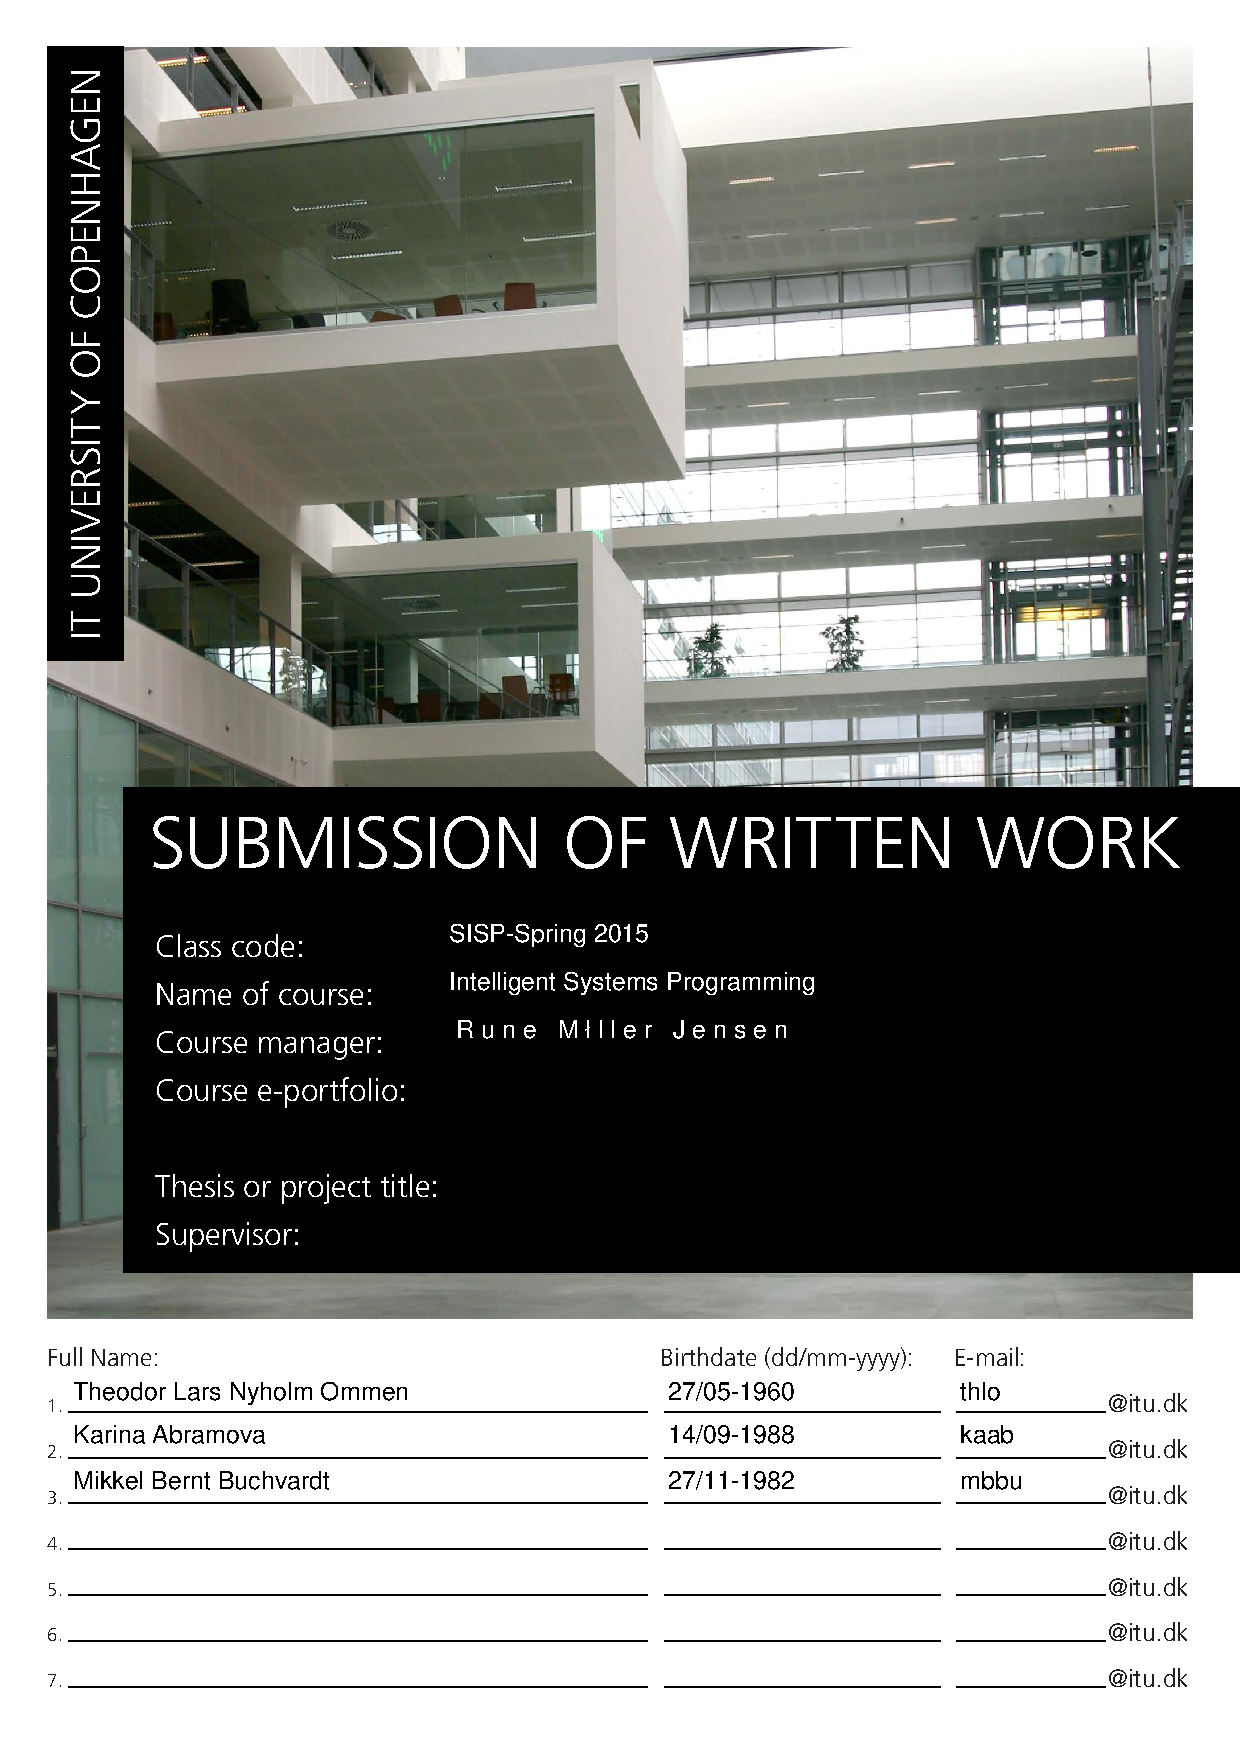
\includegraphics[scale=0.7]{./frontpage}

\begingroup
\let\flushleft
\let\endcenter\endflushleft
\maketitle
\endgroup

\section{Introduction}
The most important aspects of our implementation are:

When the solve() method is called (by user pressing the 'Solve' button in the GUI) before doing anything else all the domains are updated.

After this, the provided INITIAL\_FC() is run. If there is no consistency, the program terminates with the message "Sudoku cannot be solved". 

If there is consistency, FC() method is called. This returns the first complete assignment that it finds. 


\section{Rules}
The rules for assignments are simple - the numbers from 1 to 9 has to be exactly once in each row, in each column and in each defined square of cell size 3x3.

\section{Code}
Provided method GetRelevantVariables() is used in the method updateDomains() to traverse through all the cells in the puzzle and update their domains.
\pagebreak

After this all we needed to do was to implement the FC algorithm according to the following pseudo code:\\

FC(asn)

if asn contains no 0 then 

return asn

X $\gets$ index of first 0 in asn

Dold $\gets$D

for all V  	$\epsilon$ DX do

if AC-FC(X, V ) then 

asn[X] $\gets$ V

R $\gets$FC(asn)

if R != fail then

return R

asn[X] $\gets$ 0

D $\gets$ Dold

else

D  	$\gets$  Dold

return fail\\

The two main difficulties/bugs we encountered was the fact that the domains was copied as a hard-copy, so manipulations on D could not affect Dold. The other bug was the initialization of domains, where we first only made the domain as: {1,2,3,4,5,6,7,8,9}.
We of course were missing the 0, which indicates that the cell has not been assigned any value. 
Unfortunately, this flawed initialization of domains oddly enough made the algorithm solve the sudoku almost correctly - making the debugging extremely tedious. But of course, when we finally completely understood the AC\_FC algorithm,(and read the description of the project again), it became clear what the mistake was.

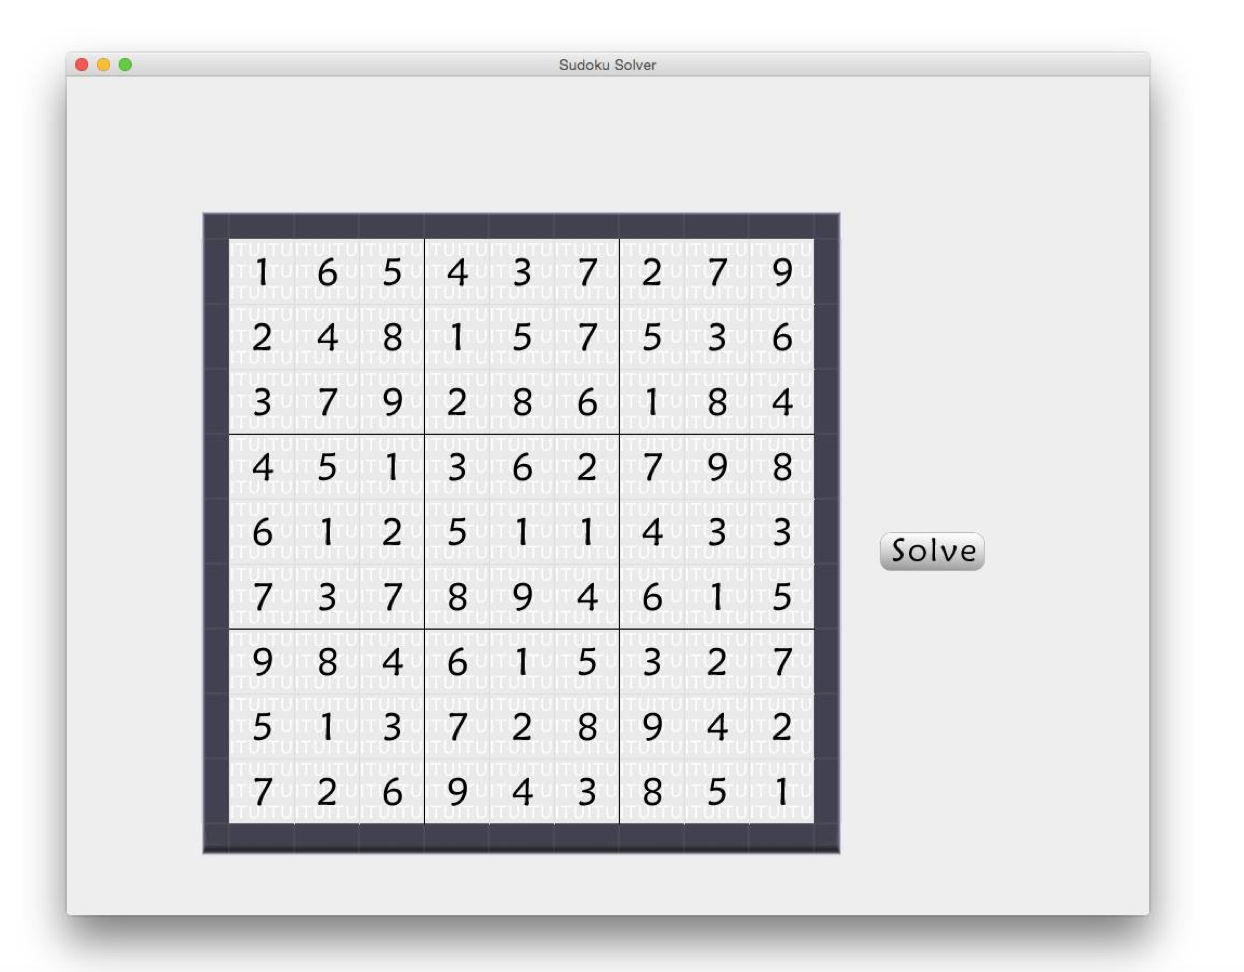
\includegraphics[scale=0.7]{./almost}

This is a picture of the “almost” solved sudoku with the domains initialized wrongly. 










\end{document}